% %%%%%%%%%%%%%%%%%%%%%%%%%%%%%%%%%%%%%%%%%%%%%%%%%%%%%%%%%%%%%%%%%%%%%%%%%%%%%%%%%
%
%	cap4.tex 
%  -----------
%
%	Neste arquivo você escreve o capítulo. Deve sempre iniciar com o ambiente
%	\chapter{Nome do Capitulo}
%
% %%%%%%%%%%%%%%%%%%%%%%%%%%%%%%%%%%%%%%%%%%%%%%%%%%%%%%%%%%%%%%%%%%%%%%%%%%%%%%%%%
%
\chapter{Metodologia}
% ----------------------------------------------------------

Esta seção apresenta a metodologia adotada para o desenvolvimento do trabalho, abrangendo a definição do modelo estrutural, a aplicação do método da rigidez para obtenção dos esforços solicitantes e os procedimentos utilizados no dimensionamento das armaduras longitudinais e transversais.

\section{Modelo Estrutural}

Para o estudo das vigas com abertura, foi escolhido um modelo de pórtico plano, em que a região do furo é formada por um quadro retangular. Essa representação permite analisar o comportamento estrutural da região da abertura e a interação entre seus elementos. A análise estrutural foi realizada pelo método da rigidez, escolhido pela facilidade de implementação computacional e pela possibilidade de aplicação a diferentes estruturas. A Figura \ref{Fig.4.1} apresenta a configuração adotada para a análise estrutural: (a) geometria da viga com abertura; (b) correspondência entre a geometria da viga e sua representação por elementos de barra; e (c) modelo de pórtico plano utilizado na análise estrutural.

\begin{figure}[htb]
    \centering
    \refstepcounter{figure}
    \label{Fig.4.1}

    \begin{minipage}{10cm}
        \fontsize{10pt}{12pt}\selectfont
        Figura \thefigure: Representação da viga com abertura e seu modelo estrutural
    \end{minipage}

    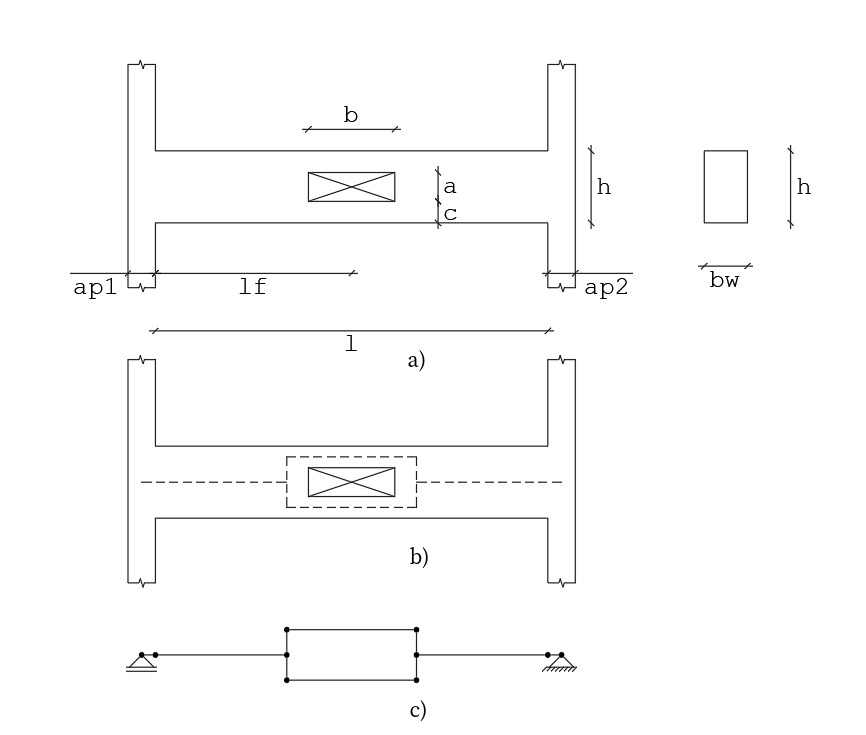
\includegraphics[scale=0.212]{modelo.png}

    \begin{minipage}{10cm}
        \fontsize{10pt}{12pt}\selectfont
        Fonte: Elaborado pelo autor (2026)
    \end{minipage}
\end{figure}

\subsection{Parâmetros Geométricos e Mecânicos do Modelo}

As barras nas regiões fora do furo têm a seção transversal da viga maciça, as seções transversais das barras que formam os banzos horizontais, superior e inferior, têm dimensões definidas a partir do desconto da região vazada.

No que diz respeito à definição da rigidez da estrutura, foi considerado o módulo de elasticidade $E_{cs}$ do concreto indicado no item 14.5.2 da \citeonline{ABNT_NBR6118_2026} para análises considerando comportamento elástico-linear do material. As barras que formam as bordas laterais do furo foram definidas com uma rigidez muito maior que a dos demais elementos, definida por um modulo de elásticidade e um momento de inércia quase infinitos. Tendo em vista que a hipótese das seções planas é válida nesta situação, estas barras devem ter, apenas, deslocamentos de corpo rígido, e deformações muito pequenas em relação às deformações do restante da estrutura. Nesse contexto, as barras foram definidas com uma seção transversal de 100x100 cm e um módulo de elasticidade de 100 $E_{cs}$.

\section{Descrição do Método da Rigidez}

Segundo \citeonline{Weaver2018}, para construir a matriz de rigidez da estrutura, é necessário obter as matrizes de rigidez dos elementos, que descrevem as relações entre as forças e os deslocamentos em cada extremidade (nós da barra), inicialmente referenciados a um sistema local de coordenadas.

Quando os elementos são expressos no sistema de coordenadas global da estrutura, os coeficientes de rigidez correspondentes aos mesmos graus de liberdade globais são somados, permitindo a montagem da matriz de rigidez da estrutura por meio da adição direta. O mesmo procedimento é aplicado à montagem do vetor de cargas equivalentes.

As matrizes de rigidez dos elementos são obtidas aplicando deslocamentos unitários (translações e rotações), individualmente, em cada grau de liberdade, mantendo os demais deslocamentos nulos. Os coeficientes $k_{ij}$ da matriz de rigidez representam a força nodal desenvolvida na direção do grau de liberdade (i) em resposta à imposição de um deslocamento unitário no grau de liberdade (j), mantendo os demais deslocamentos nodais nulos. Dessa forma, a interpretação dos índices da matriz pode ser descrita como:

\begin{enumerate}[label=\alph*)]
\item Coluna (j): identifica o grau de liberdade no qual é imposto o deslocamento unitário;
\item Linha (i): identifica o grau de liberdade no qual é determinada a força nodal correspondente.
\end{enumerate}

Na matriz de rigidez global da estrutura, o coeficiente $K_{ij}$ possui interpretação semelhante à do coeficiente $k_{ij}$ da matriz de rigidez de um elemento, porém é obtido pela montagem das matrizes de rigidez dos elementos no sistema global de coordenadas.

Na formulação do método da rigidez para um elemento de pórtico plano, são considerados três graus de liberdade por nó: duas translações (horizontal e vertical) e uma rotação. Como o elemento possui dois nós, sua formulação totaliza seis graus de liberdade. Desse modo, os vetores de forças e de deslocamentos nodais possuem dimensão 6, e o comportamento mecânico do elemento é expresso pela equação matricial \ref{eq:rigidez_barra}. A figura \ref{Fig.4.2} apresenta a matriz de rigidez de uma barra de pórtico plano no seu sistema local de coordenadas.

\begin{equation}
\mathbf{k}\mathbf{u} = \mathbf{f}
\label{eq:rigidez_barra}
\end{equation}

em que:

\begin{enumerate}[label=\alph*)]
    \item $\mathbf{k}$ = matriz de rigidez da barra no sistema de coordenadas local;
    \item $\mathbf{u}$ = vetor de deslocamentos nodais da barra no sistema de coordenadas local;
    \item $\mathbf{f}$ = vetor de forças nodais da barra no sistema de coordenadas local.
\end{enumerate}

\begin{figure}[htb]
    \centering
    \refstepcounter{figure}
    \label{Fig.4.2}

    \begin{minipage}{10cm}
        \fontsize{10pt}{12pt}\selectfont
        Figura \thefigure: Matriz de rigidez local de uma barra de pórtico plano
    \end{minipage}

    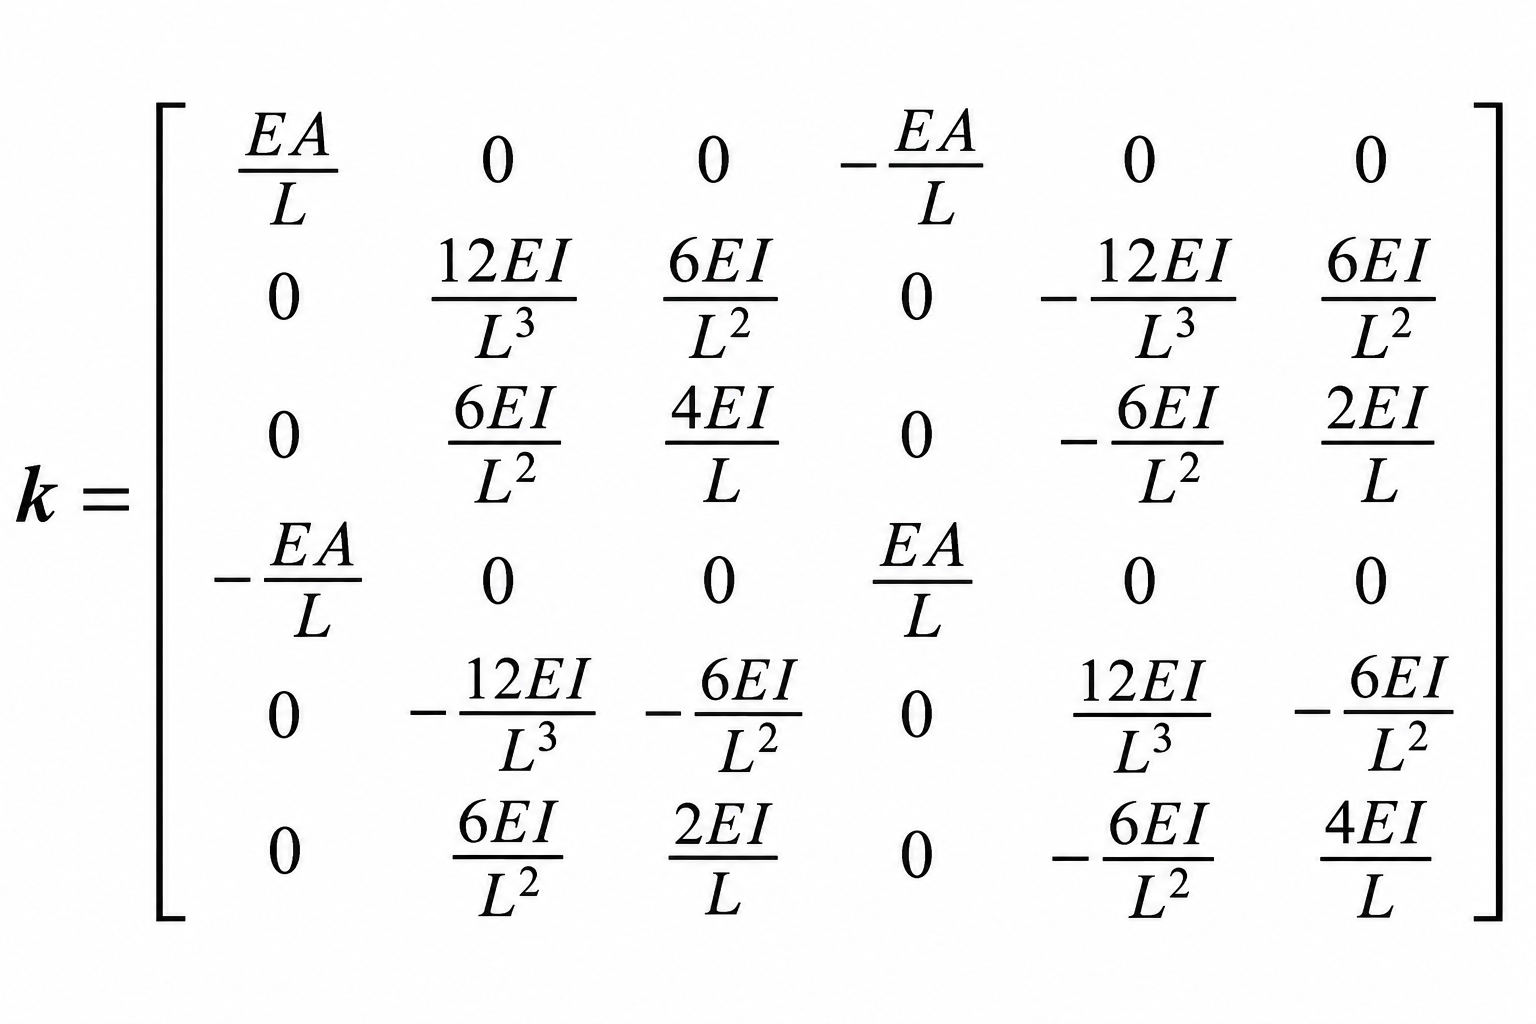
\includegraphics[scale=1.5]{matriz_barra.png}

    \begin{minipage}{10cm}
        \fontsize{10pt}{12pt}\selectfont
        Fonte: adaptado de \citeonline{Weaver2018}
    \end{minipage}
\end{figure}

\subsection{Transformação dos Sistemas de Coordenadas}

Segundo \citeonline{Weaver2018} para transformar a matriz de rigidez do elemento dos eixos locais para os eixos da estrutura, é necessária a matriz de transformação de rotação $\mathbf{R}_T$. A matriz de transformação de rotação de um pórtico plano é composta por submatrizes $R$ de rotação conforme ilustra a figura \ref{Fig.4.3}, a matriz de rotação $R$ é representada em forma expandida na figura \ref{Fig.4.4}. A matriz de transformação de rotação transposta $\mathbf{R}_T^T$ transforma os vetores de forças e deslocamentos nodais dos elementos do sistema local de coordenadas para o global, e de forma inversa a matriz $\mathbf{R}_T$ transforma os vetores do sistema global para o local conforme as equações \ref{eq:transformação_G_L} e \ref{eq:transformação_L_G}. A matriz de rigidez global da barra pode ser obtida por meio da equação \ref{eq:kG}.

\begin{equation}
\mathbf{u} = \mathbf{R}_T \mathbf{u_{G}}
\label{eq:transformação_G_L}
\end{equation}

\begin{equation}
\mathbf{u_{G}} = \mathbf{R}_T^T \mathbf{u}
\label{eq:transformação_L_G}
\end{equation}

em que:

\begin{enumerate}[label=\alph*)]
    \item $\mathbf{u_{G}}$ = vetor de deslocamentos nodais da barra no sistema de coordenadas global;
    \item $\mathbf{u}$ = vetor de deslocamentos nodais da barra no sistema de coordenadas local;
    \item $\mathbf{{R}_T}$ = matriz de transformação de rotação;
    \item $\mathbf{{R}_T^T}$ = matriz de transformação de rotação transposta.
\end{enumerate}

\begin{equation}
\mathbf{k_{G}} = \mathbf{{R}_T^T}\mathbf{k}\mathbf{{R}_T}  
\label{eq:kG}
\end{equation}

em que:

\begin{enumerate}[label=\alph*)]
    \item $\mathbf{k}$ = matriz de rigidez da barra no sistema de coordenadas local;
    \item $\mathbf{k_{G}}$ = matriz de rigidez da barra no sistema de coordenadas global;
    \item $\mathbf{{R}_T}$ = matriz de transformação de rotação;
    \item $\mathbf{{R}_T^T}$ = matriz de transformação de rotação transposta.
\end{enumerate}

\begin{figure}[htb]
    \centering
    \refstepcounter{figure}
    \label{Fig.4.3}

    \begin{minipage}{10cm}
        \fontsize{10pt}{12pt}\selectfont
        Figura \thefigure: Matriz de transformação de rotação
    \end{minipage}

    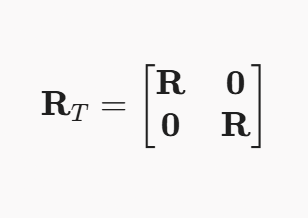
\includegraphics[scale=1]{matriz_transformação.png}

    \begin{minipage}{10cm}
        \fontsize{10pt}{12pt}\selectfont
        Fonte: adaptado de \citeonline{Weaver2018}
    \end{minipage}
\end{figure}

\begin{figure}[htb]
    \centering
    \refstepcounter{figure}
    \label{Fig.4.4}

    \begin{minipage}{10cm}
        \fontsize{10pt}{12pt}\selectfont
        Figura \thefigure: Matriz de rotação para uma barra de pórtico plano
    \end{minipage}

    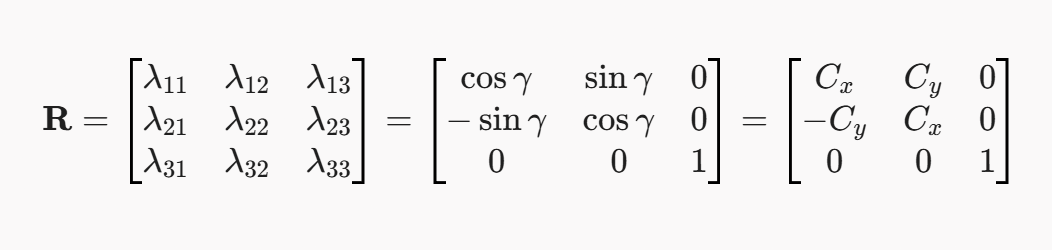
\includegraphics[scale=1]{matriz_rotação.png}

    \begin{minipage}{10cm}
        \fontsize{10pt}{12pt}\selectfont
        Fonte: adaptado de \citeonline{Weaver2018}
    \end{minipage}
\end{figure}



